\chapter{Evaluation}

In section \ref{distribution} and \ref{abstraction} it was shown that dOpenCL and Aparapi deliver satisfying performance when used on their own. Combining both libraries within Dynamic OpenCL creates the question whether the overall solution can still bring noticeable benefits to cluster computations.

For a meaningful evaluation local clusters as well as hybrid clusters will be utilized to compute diverse tasks. The employed local machine types and workloads are defined in chapter \ref{benchmarking_methodology}. In the case of cloud resources the individual capabilities will be explained in place.

\section{Local Distribution}

\subsection{Single Job Performance}
\label{single_job_performance}
In the first evaluation step a local cluster will be used to test various single workloads on one or two identical machines. Thus the combination of dOpenCL with Aparapi can be measured for speedups and potential overhead penalties of Dynamic OpenCL may be identified.

In the benchmarking setup machines of Class B are accessed from a machine of Class A through a 1 Gbit/s connection. The first test group will only contain a single machine in the cluster while for the second group two machines will be employed. At first several matrix multiplications of varying sizes are executed. The number of splits is kept equal to the number of machines. For each problem size 5 runs are taken to calculate the arithmetic mean.

\begin{figure}[H]
	
	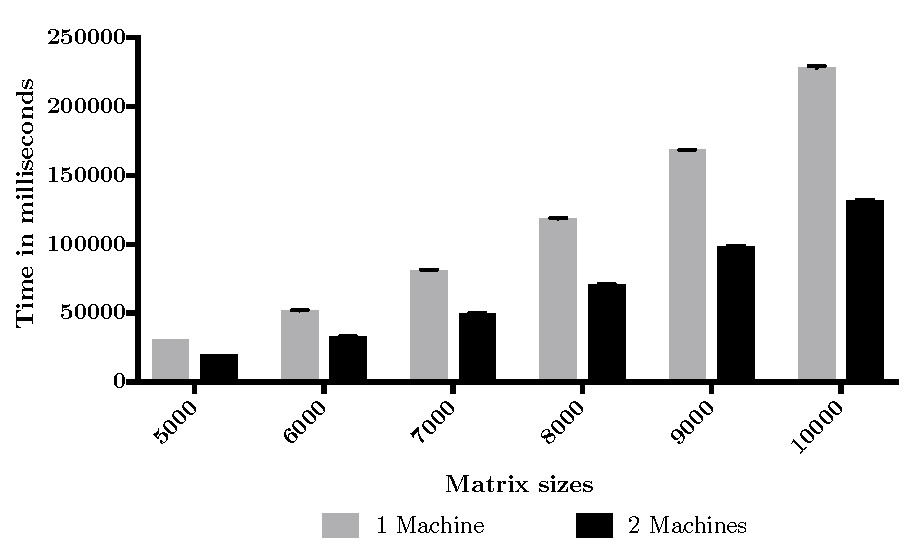
\includegraphics[width=1.0\textwidth]{images/sharded_matrix_multi.pdf}
	\centering
	\caption{Parallel Matrix Multiplication}
	\label{img:parallel_matrix}
\end{figure}

Figure \ref{img:parallel_matrix} shows that using an additional machine can lead to substantial performance benefits. It is visible that for small problem sizes the speedup is only marginal between 10-30\%. This is due to the fact that for the smaller matrix sizes the computations are executed relatively fast but are neutralized by the network interconnect that has to serve both machines at the same time. For larger matrices the ratio of computation to transferred data becomes smaller thus diminishing the network congestion effect. This can be reasoned as with rising matrix sizes of $n^2$ the computational complexity increases by $n^3$. It also becomes apparent that with growing problem sizes the speedup gets greater with a decreasing slope, which indicates that it hits a barrier around 75\%. This barrier might be imposed due to overheads by Dynamic OpenCL, Aparapi and dOpenCL but may be mainly the result of network congestions.

As matrix multiplications are computations that require noticeable amounts of data that influence the overall performance through network transfers, a second type of computation shall be evaluated that has very low data requirements. Such a workload is the Mandelbrot Set, which does not need initial data but computes values according to positions in a two dimensional array. The Mandelbrot Set was executed just as the previous matrix multiplication with 5 runs per problem size.

\begin{figure}[H]
	
	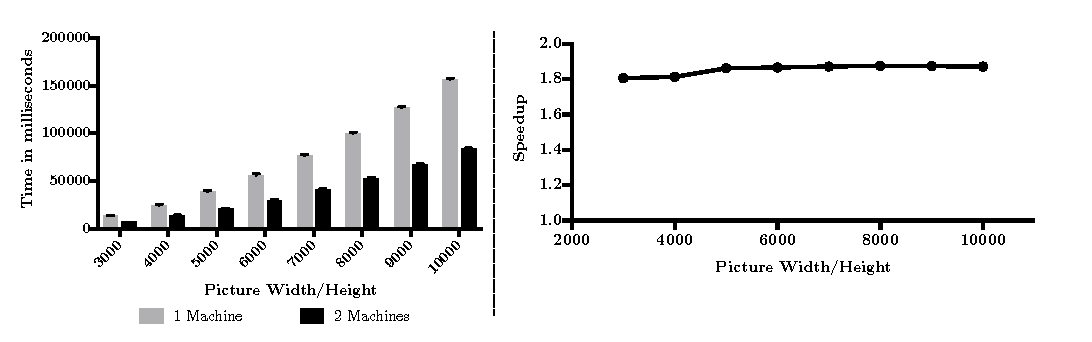
\includegraphics[width=1.0\textwidth]{images/sharded_mandelbrot.pdf}
	\centering
	\caption{Parallel Mandelbrot}
	\label{img:parallel_mandelbrot}
\end{figure}

Figure \ref{img:parallel_mandelbrot} reveals that its low data transfer requirements severely benefit the performance speedup. With speedups between 80\% and 88\% the maximum increase in performance is not only significantly higher than for the matrix multiplications but is also more stable in correlation to the problem sizes.


\subsection{Job Suite Performance}

Section \ref{single_job_performance} identified benefits when utilizing Dynamic OpenCL for a single job. In order to simulate a shared cluster environment it becomes necessary to evaluate its performance by executing variety of parallel jobs. For this reason a job suite was compiled that comprises six workloads of various complexity and type. Not only should the runtime differ per Kernel of each job but also their transferable data. The list of workloads is shown in table \ref{table:benchmark_job_setup}.

\begin{table}[!htb]
	\centering
	\begin{adjustbox}{width=0.95\textwidth}
		\small
		\begin{tabular}{l | l | l | l}
			~							& \textbf{Computational Effort}		& \textbf{Iterations}	& \textbf{Kernels per Iteration} \\
			\hline
			\textbf{Matrix Multiplication 1 (MM1)} 	& 8000x8000  								& 1 	& 5 \\
			\textbf{Matrix Multiplication 2 (MM2)}     & 6000x6000  								& 1		& 5 \\
			\textbf{Mandelbrot 1 (MB1)}     			& 1000x1000 (1000000 iterations per point) 	& 1		& 5 \\
			\textbf{Mandelbrot 2 (MB2)}     			& 2000x2000 (600000 iterations per point)  	& 1		& 5 \\
			\textbf{K-means (KM)}          			& 6000000 objects and 200 clusters  		& 10	& 1 \\
			\textbf{N-body (NB)}    		 			& 64000 objects  							& 10	& 1 \\		
		\end{tabular}
	\end{adjustbox}
	
	\caption{Benchmark Job Setup}
	\label{table:benchmark_job_setup}
\end{table}

The set of workloads thus comprises a mix of iterative and non-iterative tasks. While the iterative jobs have a fixed number of iterations and are not split per round, non-iterative tasks are split into 5 parts to enable parallelization. Although some jobs employ the same algorithm, the problem sizes are varied to create a more heterogeneous set. The implications of the problem sizes and splits for each job are explained in section \ref{workload_explanation}.

In order to prove the heterogeneity of the supplied workloads in terms of computational complexity and data transfer properties, analytical test runs are executed on a local machine of class B that measure the execution time per Kernel and the transfered data sizes. The following figure display the results of running the suite five times:

\begin{figure}[H]
	
	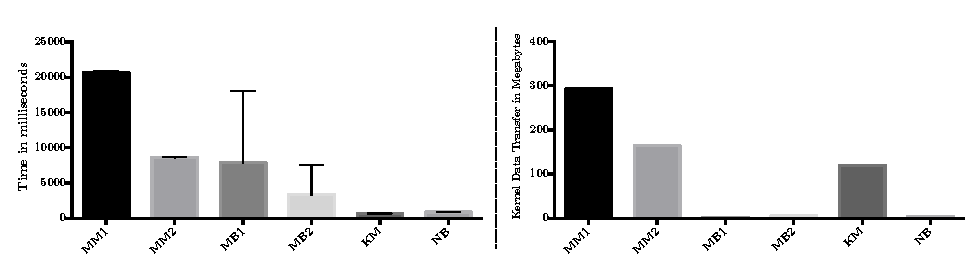
\includegraphics[width=1.0\textwidth]{images/benchmark_kernel_data_transfers.pdf}
	\centering
	\caption{Average Kernel Runtimes and Data Transfer Sizes}
	\label{img:benchmark_kernel_attributes}
\end{figure}

While it is visible that the computation times are very different, it can also be seen that the respective data transfers do not correlate to that attribute. For example, while MM2 and MB1 may require similar execution times, MM2 transfers 100x more data than MB1. The same is true for the iterative jobs KM and NB. It must be noted that MB1 and MB2 show a great standard deviation, which are not measurement errors but are a result of the nature of the algorithm. Mandelbrot calculations can not be split evenly in terms of computational effort and instead may run some Kernels for long times while having virtually no computations required by other Kernels.

For the benchmark the performance indicator to measure is the total time to finish all tasks. As the selection of scheduling algorithms has a big impact on this value, it is necessary to define the utilized algorithms. For the job scheduling tier a round robin approach is used. On the device scheduling level a historic performance based algorithm is used that assigns a Kernel to the best performing device in case multiple are available. In order to allow for a fair comparison among multiple runs, all jobs are submitted before starting the execution engine.

The suite is executed five times on three different cluster setups. At first it is executed on a single machine of class B. In this setup no network transfer is needed as the management node also executed the Kernels. For the second cluster a machine of class B is added, which is connected by a 10 Gbit/s interconnect. Therefore, some Kernels may have to be sent over the network while others will be executed directly on the management node. In the final run another machine of class A is added, which is only connected with 1 Gbit/s but has a very high computational capability. The results of the benchmark are visible in the following figure:

\begin{figure}[H]
	
	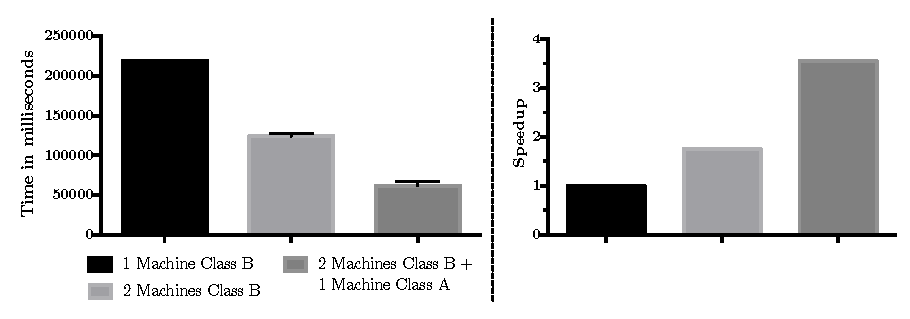
\includegraphics[width=1.0\textwidth]{images/local_full_benchmark_results.pdf}
	\centering
	\caption{Local Benchmark Results}
	\label{img:local_benchmark_results}
\end{figure}

The results indicate that employing a second machine that is connected through a fast Ethernet connection can produce significant performance benefits. Although Kernels have to be sent over the network to the second machine, it still yields an average speedup of x1.76. It also reveals that the scheduling works sufficiently even though it is based on naive algorithms. In the last cluster setup the high performance machine of class A is added, which is connected only by 1 Gbit/s. Even though the network slows down the execution times on this machine it can still double the performance of the cluster, leading to a speedup of x3.54. Thus it can be concluded that the parallelization by Dynamic OpenCL through remote machines is a viable option within a local cluster. It has to be noted though that high performance machines like machines of class A may be underutilized and slowed down by network transfers.

\section{Hybrid Distribution}


mention utilized aws region